\chapter{Fourier Series of a Square Wave}
\label{sec:squareWaveFourierSeries}

Consider a square wave $f(t)$ of amplitude $a$ and period $L$. An example is
shown in~\cref{fig:squareWave}.

\begin{figure}[h]
  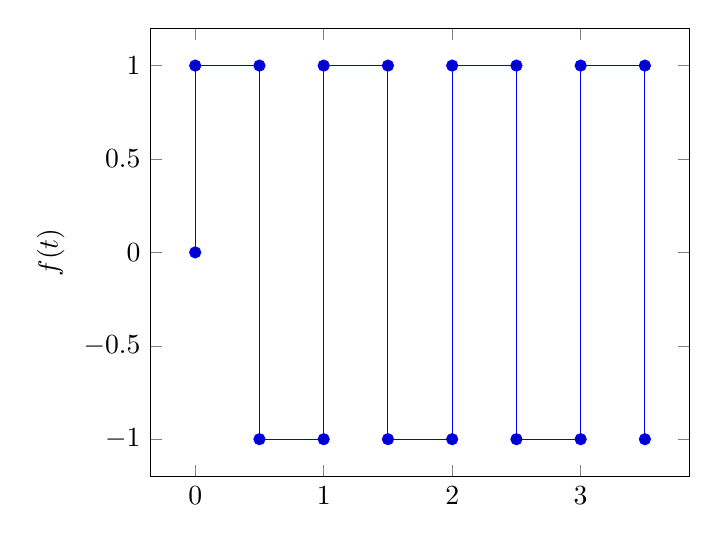
\begin{tikzpicture}
    \begin{axis}[ylabel=$f(t)$]
      \addplot +[const plot] coordinates {(0,0) (0,1) (0.5,1) (0.5,-1)
      (1,-1) (1,1) (1.5,1) (1.5,-1) (2,-1) (2,1) (2.5,1) (2.5,-1) (3,-1) (3,1)
    (3.5, 1)(3.5,-1)};
    \end{axis}
  \end{tikzpicture}
  \caption[Square wave]{Square wave with amplitude $1$ and frequency $\SI{1}{\Hz}$}
  \label{fig:squareWave}
\end{figure}

Now by any good mathematical methods textbook (in this case, we cite the
excellent \textcite{FourierSeries}), a periodic function\footnote{Strictly, the
  function must meet a number of conditions, called the Dirichlet criteria, but
we shall just take it as a given that the square wave does meet all of these
(the proof of each of them is essentially trivial depending upon your definition
of a square wave)} $f(x)$ can be represented by the following series (known as a
Fourier series)

\begin{equation*}
  f(x) = \frac{a_0}{2} + \sum_{r=1}^{\infty} \left[ a_r\cos\left(\frac{2\pi rx}{L}\right) + b_r\sin\left(\frac{2\pi rx}{L}\right)\right]
\end{equation*}

where

\begin{eqnarray*}
  a_r &=& \frac{2}{L} \int_{x_0}^{x_0+L} f(x)\cos\left(\frac{2\pi rx}{L}\right)\,\mathrm{d}x\\
  b_r &=& \frac{2}{L} \int_{x_0}^{x_0+L} f(x)\sin\left(\frac{2\pi rx}{L}\right)\,\mathrm{d}x
\end{eqnarray*}

where $x_0$ is arbitrary and $L$ is the period of the function.

A handy time-saving trick is to realise that the square wave is an odd function
(i.e., $\forall x\: f(-t)=-f(t)$) so there will be no cosine terms in the series
(again, this needs to be made more rigorous, but see a maths textbook) and so
$a_r=0$.

To evaluate $b_r$, we take $t_0=-\frac{L}{2}$ and split up the integral into two
parts. From $-\frac{L}{2}$ to $0$ $f(t)=-a$ and from $0$ to
$\frac{L}{2}$ $f(t)=+a$.  We then have

\begin{equation*}
  \int_{-\frac{L}{2}}^{\frac{L}{2}} f(t)\sin\left(\frac{2\pi rt}{L}\right)\,\mathrm{d}t
  = a\int_{-\frac{L}{2}}^0 -\sin\left(\frac{2\pi rt}{L}\right)\,\mathrm{d}t + a\int_0^{\frac{L}{2}} \sin\left(\frac{2\pi rt}{L}\right)\,\mathrm{d}t\\
\end{equation*}

which, using the substitution $u=-t$ on the left integral, equals

\begin{equation*}
  2a\int_0^{\frac{L}{2}} \sin\left(\frac{2\pi rt}{L}\right)\,\mathrm{d}t
  = \frac{aL}{\pi r} \left[\cos\left(\frac{2\pi rt}{L}\right)\right]_{\frac{L}{2}}^0
  = \frac{aL}{\pi r}\left[1-\cos\left(\pi r\right)\right]
\end{equation*}

Noting that $\cos 0\pi = 1$, $\cos 1\pi = -1$, $\cos 2\pi=1$ and so on, we obtain

\begin{equation*}
  b_r = \frac{2a}{\pi r}\left[1-(-1)^r\right]
   = \begin{cases}
       r\text{ even} &  0\\
       r\text{ odd} & \frac{4a}{\pi r}
     \end{cases}
\end{equation*}

and hence

\begin{equation*}
  \boxed{f(t) = \frac{4a}{\pi}\left(\sin \omega t + \frac{\sin 3\omega t}{3} + \frac{\sin 5\omega t}{5} + \dots \right)}
\end{equation*}

where the angular frequency $\omega = \frac{2\pi}{L}$. Plotting the first terms
of this equation gives the various graphs shown
in~\cref{fig:squareWaveApproximations}.
